% =============================================================================
\section{Volar con comandos}
% =============================================================================

\begin{frame}{Offboard contra comandos}
  \begin{columns}[t]
    \column{0.48\textwidth}\centering
    \begin{tikzpicture}[every node/.style={font=\scriptsize,align=center}]
      \node (d) at (0,0) {\dronarriba{1.3cm}};
      \foreach \i in {1,...,6} \draw[-{Stealth},naranja,thick] (-2.6,1.1-\i*0.35) -- (-0.9,1.1-\i*0.35);
      \node[draw=naranja,fill=yellow!20,rounded corners] at (-3.6,0) {tu nodo};
    \end{tikzpicture}\\[0.3em]
    \textbf{Offboard: ``sigue mi mano''}\\[0.2em]
    \small Tu nodo manda dónde estar \textbf{10 veces por segundo}. Tú diseñas la trayectoria. Si te callas,
    PX4 pasa a Hold.
    \column{0.48\textwidth}\centering
    \begin{tikzpicture}[every node/.style={font=\scriptsize,align=center}]
      \node (d) at (0,0) {\dronarriba{1.3cm}};
      \draw[-{Stealth},naranja,line width=2pt] (-2.6,0) -- (-0.9,0);
      \node[draw=naranja,fill=yellow!20,rounded corners] at (-3.6,0) {tu nodo};
      \node[font=\tiny,text=naranja] at (-1.75,0.35) {una orden};
    \end{tikzpicture}\\[0.3em]
    \textbf{Comandos: ``ve a tal lugar''}\\[0.2em]
    \small Tu nodo manda \textbf{una orden} (despega, ve a este punto GPS, regresa) y PX4 la ejecuta con sus
    propias maniobras. Si te callas, sigue con lo último que le pediste.
  \end{columns}
  \vspace{0.6em}
  \begin{idea}
    \small Comandos = lo mismo que los botones de QGC, pero desde tu código. Más simple y más seguro; menos
    control fino.
  \end{idea}
\end{frame}

\begin{frame}{VehicleCommand: un formulario con 7 casillas}
  \begin{columns}[c]
    \column{0.42\textwidth}\centering
    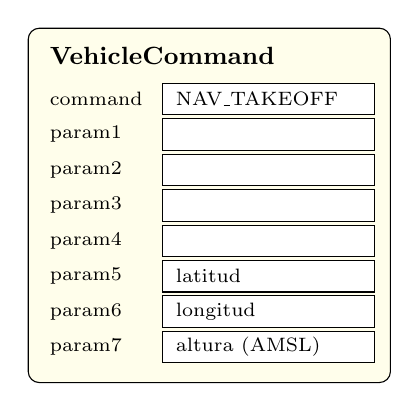
\begin{tikzpicture}[every node/.style={font=\scriptsize,anchor=west}]
      \draw[fill=yellow!8,rounded corners] (0,-0.2) rectangle (4.6,4.3);
      \node[font=\small\bfseries] at (0.15,3.95) {VehicleCommand};
      \node at (0.15,3.4) {\cmd{command}}; \draw[fill=white] (1.7,3.2) rectangle (4.4,3.6); \node at (1.75,3.4) {\cmd{NAV\_TAKEOFF}};
      \foreach \i/\v in {1/,2/,3/,4/,5/latitud,6/longitud,7/altura (AMSL)} {
        \node at (0.15,3.4-\i*0.45) {\cmd{param\i}};
        \draw[fill=white] (1.7,3.2-\i*0.45) rectangle (4.4,3.6-\i*0.45);
        \node at (1.75,3.4-\i*0.45) {\v};}
    \end{tikzpicture}
    \column{0.55\textwidth}\small
    \begin{itemize}
      \item \cmd{command} dice \textbf{qué hacer}; los 7 \cmd{param} son los detalles. Cada comando usa los suyos.
      \item Una casilla que no aplica va en \cmd{NaN} (``no me importa'') o en 0.
    \end{itemize}
    \centering\scriptsize
    \begin{tabular}{ll}
      \toprule
      Comando & Casillas \\
      \midrule
      \cmd{COMPONENT\_ARM\_DISARM} & p1: 1 armar, 0 desarmar \\
      \cmd{DO\_SET\_MODE} & p1 = 1, p2: modo (6 = Offboard) \\
      \cmd{NAV\_TAKEOFF} & p5--p7: dónde y a qué altura \\
      \cmd{DO\_REPOSITION} & p1 velocidad, p5--p7: a dónde \\
      \cmd{NAV\_LAND} & ninguna \\
      \cmd{NAV\_RETURN\_TO\_LAUNCH} & ninguna \\
      \bottomrule
    \end{tabular}
  \end{columns}
\end{frame}

\begin{frame}{¿Me hizo caso? El ack}
  \centering
  \begin{tikzpicture}[every node/.style={font=\scriptsize,align=center}]
    \node[draw=naranja,fill=yellow!20,rounded corners,minimum height=1cm] (n) at (0,0) {tu nodo};
    \node (d) at (7,0) {\dronarriba{1.6cm}};
    \draw[-{Stealth},thick,naranja] (1,0.3) -- node[above]{\cmd{vehicle\_command}: ``arma''} (6,0.3);
    \draw[{Stealth}-,thick,verde] (1,-0.3) -- node[below]{\cmd{vehicle\_command\_ack}: ACCEPTED o DENIED} (6,-0.3);
  \end{tikzpicture}
  \vspace{0.6em}

  \begin{columns}[c]
    \column{0.5\textwidth}
    \begin{terminal}{goto\_mission}
PX4 rechazó el comando 400 (result=1)
    \end{terminal}
    \column{0.47\textwidth}\small
    \begin{itemize}
      \item PX4 contesta cada comando. \cmd{result = 0} es \textbf{aceptado}; otro número, rechazado.
      \item 400 = armar. ¿Por qué lo rechazó? QGC y \cmd{flight\_mode\_monitor} dicen la razón.
      \item Los ejemplos con comandos \textbf{reintentan} cada segundo: al arrancar, PX4 a veces aún no está
        listo.
    \end{itemize}
  \end{columns}
\end{frame}

% -----------------------------------------------------------------------------
\begin{frame}{goto\_mission paso a paso}
  \begin{columns}[c]
    \column{0.45\textwidth}\centering
    \begin{tikzpicture}[scale=0.58]
      \draw[gray!25,step=1] (-1.4,-1.4) grid (6.4,6.4);
      \draw[-{Stealth},verde,thick] (0,-1.4) -- (0,6.6) node[above,font=\tiny] {N};
      \draw[-{Stealth},rojo,thick] (-1.4,0) -- (6.6,0) node[right,font=\tiny] {E};
      \fill[verde!60] (-0.5,-0.5) rectangle (0.5,0.5); \node[font=\tiny\bfseries,text=white] at (0,0) {H};
      \foreach \e/\n/\l in {0/5/0,5/5/1,5/0/2} {\fill[naranja] (\e,\n) circle (3.5pt); \node[font=\tiny\bfseries,above right] at (\e,\n) {WP\l};}
      \node[font=\tiny\bfseries,below right] at (0.3,-0.3) {WP3};
      \draw[azul,line width=2pt,visible on=<5->] (0,0) -- (0,5);
      \draw[azul,line width=2pt,visible on=<6->] (0,5) -- (5,5) -- (5,0) -- (0,0);
      \draw[azul,dashed,thick,-{Stealth},visible on=<4>] (0,0.7) -- (0,4.5);
      \draw[azul,dashed,thick,-{Stealth},visible on=<5>] (0.6,5) -- (4.5,5);
      \only<1-4,6-7>{\node at (0,0) {\dronarriba{0.85cm}};}
      \only<5>{\node at (0,5) {\dronarriba{0.85cm}};}
      \draw[gray] (8,0) -- (8,6); \node[font=\tiny,text=gris] at (8,6.4) {altura};
      \foreach \h in {0,5} \draw[gray] (7.85,\h) -- (8.15,\h) node[right,font=\tiny,text=gris] {\h\,m};
      \only<1-2,7>{\fill[azul] (8,0) circle (5pt);}
      \only<4-5>{\fill[azul] (8,5) circle (5pt);}
      \only<3>{\draw[-{Stealth},line width=2pt,verde] (8,0.2) -- (8,4.8);}
      \only<6>{\draw[-{Stealth},line width=2pt,naranja] (8,4.8) -- (8,0.2);}
    \end{tikzpicture}
    \column{0.53\textwidth}
    \begin{tikzpicture}[every node/.style={font=\tiny\bfseries,rounded corners,minimum width=1.15cm,minimum height=0.5cm,draw=azul}]
      \node[alt=<1>{fill=yellow!60}{fill=azulclaro}] at (0,0) {WAIT\_GPS};
      \node[alt=<2>{fill=yellow!60}{fill=azulclaro}] at (1.3,0) {ARMING};
      \node[alt=<3>{fill=yellow!60}{fill=azulclaro}] at (2.6,0) {TAKEOFF};
      \node[alt=<4-5>{fill=yellow!60}{fill=azulclaro}] at (3.9,0) {GOTO};
      \node[alt=<6>{fill=yellow!60}{fill=azulclaro}] at (5.2,0) {RETURN};
      \node[alt=<7>{fill=yellow!60}{fill=azulclaro}] at (6.5,0) {DONE};
    \end{tikzpicture}
    \vspace{0.3em}

    \only<1>{\begin{terminal}{goto\_mission}
goto\_mission: esperando posición GPS...\\
GPS listo, armando
    \end{terminal}\small Espera a que PX4 sepa dónde está (latitud y longitud válidas). Guarda ese punto como
      \textbf{casa}.}%
    \only<2>{\begin{terminal}{goto\_mission}
(cada segundo: Hold, luego armar)
    \end{terminal}\small Pide modo \textbf{Hold} y luego \textbf{armar}, y reintenta cada segundo hasta que PX4
      dice que sí. Nada de setpoints: aquí no hay Offboard.}%
    \only<3>{\begin{terminal}{goto\_mission}
Armado, despegando a 5.0 m
    \end{terminal}\small Un solo \cmd{NAV\_TAKEOFF}. PX4 sube solo y al llegar se queda en Hold.}%
    \only<4>{\begin{terminal}{goto\_mission}
Yendo al WP 0: 5.0 m N, 0.0 m E\\
WP 0 a 3.2 m
    \end{terminal}\small Convierte ``5 m al norte'' a latitud y longitud y manda un \cmd{DO\_REPOSITION}. PX4
      vuela hasta allá.}%
    \only<5>{\begin{terminal}{goto\_mission}
Llegué al WP 0\\
Yendo al WP 1: 5.0 m N, 5.0 m E
    \end{terminal}\small Mide la distancia con la posición local; a menos de 0.5 m manda el siguiente. Una orden
      por waypoint, no 10 por segundo.}%
    \only<6>{\begin{terminal}{goto\_mission}
Llegué al WP 3\\
Misión completa, regresando a casa
    \end{terminal}\small Al terminar, \cmd{NAV\_RETURN\_TO\_LAUNCH}: PX4 regresa y aterriza solo.}%
    \only<7>{\begin{terminal}{goto\_mission}
En casa y desarmado
    \end{terminal}\small PX4 desarmó al tocar tierra. Fin.}%
  \end{columns}
\end{frame}

\begin{frame}{De metros a GPS}
  \begin{columns}[c]
    \column{0.45\textwidth}\centering
    \begin{tikzpicture}
      \draw[gray!50] (0,0) circle (1.8);
      \draw[gray!50] (-1.8,0) arc (180:360:1.8 and 0.5);
      \draw[gray!50,dashed] (-1.8,0) arc (180:0:1.8 and 0.5);
      \draw[gray!50] (0,-1.8) arc (-90:90:0.7 and 1.8);
      \fill[naranja] (0.55,1.0) circle (2.5pt) node[right,font=\tiny] {casa};
      \fill[azul] (0.55,1.35) circle (2.5pt) node[right,font=\tiny] {WP: 5 m al norte};
      \draw[-{Stealth},thick] (0.55,1.05) -- (0.55,1.3);
    \end{tikzpicture}
    \column{0.52\textwidth}\small
    \cmd{DO\_REPOSITION} pide \textbf{latitud y longitud}, no metros. Desde casa:
    \[
      \text{lat} = \text{lat}_0 + \frac{\text{norte}}{R}\cdot\frac{180}{\pi}
      \qquad
      \text{lon} = \text{lon}_0 + \frac{\text{este}}{R\cos(\text{lat}_0)}\cdot\frac{180}{\pi}
    \]
    con $R = 6\,371\,000$ m (radio de la Tierra).
    \begin{itemize}
      \item 1 grado de latitud $\approx$ 111 km: 5 m son \textasciitilde0.000045°.
      \item Por eso la latitud se guarda en \cmd{double}: en \cmd{float} se pierden los metros.
    \end{itemize}
  \end{columns}
\end{frame}

\begin{frame}[fragile]{return\_home: aléjate y regresa}
  \begin{columns}[c]
    \column{0.5\textwidth}\centering
    \begin{tikzpicture}[scale=0.6]
      \fill[green!35!black!40] (-0.8,-0.2) rectangle (8.6,0);
      \fill[verde] (0,0) circle (4pt) node[below=3pt,font=\tiny] {casa};
      \draw[gray!50] (-0.6,0) -- (-0.6,6.2);
      \foreach \h/\l in {1.2/5,6/30} \draw[gray!50] (-0.7,\h) -- (-0.5,\h) node[left,font=\tiny,text=gris] {\l\,m};
      \draw[azul,thick,-{Stealth},visible on=<1->] (0,0.3) -- (0,1.2) -- (7.4,1.2);
      \draw[naranja,thick,-{Stealth},visible on=<2->] (7.6,1.4) -- (7.6,6);
      \draw[naranja,thick,-{Stealth},visible on=<3->] (7.4,6) -- (0.2,6);
      \draw[naranja,thick,-{Stealth},visible on=<4->] (0,5.8) -- (0,0.3);
      \only<1>{\node at (7.6,1.2) {\dronlado{1.1cm}};}
      \only<2>{\node at (7.6,6) {\dronlado{1.1cm}};}
      \only<3>{\node at (2.5,6) {\dronlado{1.1cm}};}
      \only<4>{\node[anchor=south] at (0,0) {\dronlado{1.1cm}};}
      \node[font=\tiny,text=gris] at (4,0.6) {36 m};
    \end{tikzpicture}
    \column{0.47\textwidth}
    \only<1>{\begin{terminal}{return\_home}
Alejándome 30 m N, 20 m E
    \end{terminal}\small Despega a 5 m y se aleja con \cmd{DO\_REPOSITION}.}%
    \only<2>{\begin{terminal}{return\_home}
Lejos de casa (36 m). Return!\\
subiendo a la altura de retorno\\
\ \ | a 35.8 m de casa, altura 12.4 m
    \end{terminal}\small Manda \cmd{NAV\_RETURN\_TO\_LAUNCH}. Lo primero que hace PX4 es \textbf{subir} a la
      altura de retorno (30 m en el x500 de SITL) para no chocar con nada.}%
    \only<3>{\begin{terminal}{return\_home}
volando a casa | a 21.4 m de casa,\\
\ \ altura 30.0 m
    \end{terminal}\small Vuela en línea recta hacia casa, a esa altura.}%
    \only<4>{\begin{terminal}{return\_home}
sobre casa, bajando | a 0.4 m de casa,\\
\ \ altura 8.7 m\\
En casa y desarmado (a 0.3 m del home)
    \end{terminal}\small Baja, aterriza y desarma solo. Es lo mismo que pasa con batería baja o si se pierde la
      conexión.}%
  \end{columns}
\end{frame}

\begin{frame}{Los otros comandos}
  \centering
  \begin{tikzpicture}[every node/.style={font=\scriptsize,align=center},
      cd/.style={draw=azul,fill=azulclaro,rounded corners,text width=5.6cm,minimum height=1.5cm}]
    \node[cd] at (0,1.0) {\textbf{orbit\_command}\\PX4 vuela el círculo solo (\cmd{DO\_ORBIT}). Compáralo con
      \cmd{orbit\_mission}, donde lo calculabas tú.};
    \node[cd] at (6.4,1.0) {\textbf{change\_speed}\\Cambia la velocidad en pleno vuelo
      (\cmd{DO\_CHANGE\_SPEED}).};
    \node[cd] at (0,-0.8) {\textbf{set\_home}\\Mueve la ``casa'' a otro punto: Return regresa ahí
      (\cmd{DO\_SET\_HOME}).};
    \node[cd,fill=red!5,draw=rojo] at (6.4,-0.8) {\textbf{motor\_test}\\Prueba un motor a la vez, en tierra
      (\cmd{ACTUATOR\_TEST}). En el real: \textbf{sin hélices}.};
  \end{tikzpicture}
  \vspace{0.6em}

  \raggedright\small
  \begin{tabular}{@{}ll@{}}
    \textbf{¿Offboard?} & trayectorias tuyas, reaccionar rápido a sensores (seguir algo, esquivar). \\
    \textbf{¿Comandos?} & ir de un punto a otro, despegar, aterrizar, regresar. Si un comando hace lo que
      necesitas, úsalo.
  \end{tabular}
\end{frame}
